\chapter{Design}
\label{ch:design}

In this chapter, we describe the overall design of our PIO device, and how we plan to integrate it into a RISC-V SoC.

\section{PIO Assembly}
\label{sec:pioasm}

The design of the PIO starts with the assembly language which it executes. We reuse parts of the assembly language from the RP2040 PIO, as described in section 3.3 of the RP2040 Datasheet and shown in Table \ref{tab:pioasm}. There are 9 instructions, each 16 bits long. The upper 3 bits are the opcode, and bits 12-8 encode a delay and/or side set, the functionality of which are described in Section \ref{sec:functionality}. The rest of the instructions differ, encoding different flags and data. We omit the full description of the original PIO instruction set for brevity, instead referring to the datasheet \cite{rp2040}.

\begin{table}[h!]
    \centering
    \begin{tabular}{|c|c|c|c|c|c|c|c|c|c|c|c|c|c|c|c|c|}
        \hline
        Bit:       & 15 & 14 & 13 & 12                                  & 11                               & 10                             & 9                           & 8                          & 7 & 6 & 5 & 4 & 3 & 2 & 1 & 0 \\ \hline
        \txt{JMP}  & 0  & 0  & 0  & \multicolumn{5}{c|}{Delay/side-set} & \multicolumn{3}{c|}{Condition}   & \multicolumn{5}{c|}{Address}                                                                                              \\ \hline
        \txt{WAIT} & 0  & 0  & 1  & \multicolumn{5}{c|}{Delay/side-set} & Pol                              & \multicolumn{2}{c|}{Source}    & \multicolumn{5}{c|}{Index}                                                               \\ \hline
        \txt{IN}   & 0  & 1  & 0  & \multicolumn{5}{c|}{Delay/side-set} & \multicolumn{3}{c|}{Source}      & \multicolumn{5}{c|}{Bit count}                                                                                            \\ \hline
        \txt{OUT}  & 0  & 1  & 1  & \multicolumn{5}{c|}{Delay/side-set} & \multicolumn{3}{c|}{Destination} & \multicolumn{5}{c|}{Bit count}                                                                                            \\ \hline
        \txt{PUSH} & 1  & 0  & 0  & \multicolumn{5}{c|}{Delay/side-set} & 0                                & IfE                            & Blk                         & 0                          & 0 & 0 & 0 & 0                 \\ \hline
        \txt{PULL} & 1  & 0  & 0  & \multicolumn{5}{c|}{Delay/side-set} & 1                                & IfE                            & Blk                         & 0                          & 0 & 0 & 0 & 0                 \\ \hline
        \txt{MOV}  & 1  & 0  & 1  & \multicolumn{5}{c|}{Delay/side-set} & \multicolumn{3}{c|}{Destination} & \multicolumn{2}{c|}{Op}        & \multicolumn{3}{c|}{Source}                                                              \\ \hline
        \txt{IRQ}  & 1  & 1  & 0  & \multicolumn{5}{c|}{Delay/side-set} & 0                                & Clr                            & Wait                        & \multicolumn{5}{c|}{Index}                                 \\ \hline
        \txt{SET}  & 1  & 1  & 1  & \multicolumn{5}{c|}{Delay/side-set} & \multicolumn{3}{c|}{Destination} & \multicolumn{5}{c|}{Data}                                                                                                 \\ \hline
    \end{tabular}
    \caption{The RP2040 PIO assembly language \cite{rp2040}}
    \label{tab:pioasm}
\end{table}

Our version of pioasm is much simplified from this: the number of instructions is reduced from 9 to 8, some of the flags are removed, and much of the functionality of the instructions that is configurable via registers is instead fixed. These restrictions are necessary to simplify the design such that it can be implemented within a realistic timeframe. Our PIO instruction set, referred to as RVPIO (RISC-V PIO) from here on, is shown in Table \ref{tab:rvpioasm} as a proof of concept, and details of the changes between the two are given below.

\begin{itemize}
    \item The \txt{IRQ} instruction is removed. This is to simplify integration of the PIO into the SoC: handling interrupts in either direction is a very involved process on both the hardware and software level and is left out of scope for this project.
    \item Bit 12 is always side-set, and only 1 pin may be set/cleared using this. The side-set pin is fixed in the hardware.
    \item The \txt{WAIT} instruction can only wait on an input pin changing state, instead of being configurable to wait on an \txt{IRQ} instead. The pin that is waited on is selected by an instruction operand.
    \item \txt{IN} and \txt{OUT} instructions are reduced in the sources/destinations they can shift from/to. They may only shift to/from a scratch register or pins. The \txt{OUT} instruction can not shift to the program counter or execute OSR data as an instruction.
    \item \txt{PUSH} and \txt{PULL} instructions do not have the block (Blk) flag, instead behaving as if this flag was always set, which is to stall execution if the FIFO is full/empty.
    \item \txt{MOV} is restricted in it's capabilities. The original optionally could invert or reverse the bits of the data before writing, which is not implemented in RVPIO. The sources/destinations are also restricted: it cannot read from status registers, and it cannot write to the program counter or execute data as an instruction.
    \item \txt{MOV}, \txt{SET}, and \txt{OUT} include a `pindirs' output location in the RP2040, which allows to change the pin mapping during the execution of a program. This is not available in RVPIO, pin mapping is controllable only via the control registers.
\end{itemize}

\begin{table}[h!]
    \centering
    \begin{tabular}{|c|c|c|c|c|c|c|c|c|c|c|c|c|c|c|c|c|}
        \hline
        Bit:       & 15 & 14 & 13 & 12   & 11                         & 10                               & 9                              & 8 & 7                               & 6 & 5 & 4 & 3 & 2 & 1 & 0 \\ \hline
        \txt{JMP}  & 0  & 0  & 0  & S.S. & \multicolumn{4}{c|}{Delay} & \multicolumn{3}{c|}{Condition}   & \multicolumn{5}{c|}{Address}                                                                     \\ \hline
        \txt{WAIT} & 0  & 0  & 1  & S.S. & \multicolumn{4}{c|}{Delay} & Pol                              & 0                              & 0 & \multicolumn{5}{c|}{Pin Select}                             \\ \hline
        \txt{IN}   & 0  & 1  & 0  & S.S. & \multicolumn{4}{c|}{Delay} & \multicolumn{3}{c|}{Source}      & \multicolumn{5}{c|}{Bit count}                                                                   \\ \hline
        \txt{OUT}  & 0  & 1  & 1  & S.S. & \multicolumn{4}{c|}{Delay} & \multicolumn{3}{c|}{Destination} & \multicolumn{5}{c|}{Bit count}                                                                   \\ \hline
        \txt{PUSH} & 1  & 0  & 0  & S.S. & \multicolumn{4}{c|}{Delay} & 0                                & IfE                            & 0 & 0                               & 0 & 0 & 0 & 0             \\ \hline
        \txt{PULL} & 1  & 0  & 0  & S.S. & \multicolumn{4}{c|}{Delay} & 1                                & IfE                            & 0 & 0                               & 0 & 0 & 0 & 0             \\ \hline
        \txt{MOV}  & 1  & 0  & 1  & S.S. & \multicolumn{4}{c|}{Delay} & \multicolumn{3}{c|}{Destination} & 0                              & 0 & \multicolumn{3}{c|}{Source}                                 \\ \hline
        \txt{SET}  & 1  & 1  & 1  & S.S. & \multicolumn{4}{c|}{Delay} & \multicolumn{3}{c|}{Destination} & \multicolumn{5}{c|}{Data}                                                                        \\ \hline
    \end{tabular}
    \caption{Our RVPIO assembly language \cite{rp2040}}
    \label{tab:rvpioasm}
\end{table}


\section{Functional Details}
\label{sec:functionality}

The assembly language informs most of the implementation details of RVPIO, but there are some other details which must be clarified so that we may define the set of control registers and the details of how different system components will interact before we move to implementation. Again, most of these details are drawn from the RP2040 datasheet \cite{rp2040} and modified/simplified to reduce complexity.

Side-set is a feature of the PIO that allows for instructions to encode data to write to the pins directly within them. When an instruction is executed, the side-set value is written immediately to pre-configured output pins. This is useful for, for example, driving a clock signal on each cycle in parallel with writing out data. In RVPIO, only one side-set bit may be encoded in each instruction, and there is a fixed output pin for side-set.

Delays encoded into instructions allow to more precisely control the timing of a program. Certain instructions may need to be executed on certain cycles, so delays allow to tell the system to optionally insert a number of cycles of delay after the execution of an instruction, on top of the single cycle it takes to execute instructions usually. Up to 16 cycles of delay may be included after each RVPIO instruction.

As shown in Figure \ref{fig:pio-sm}, the PIO includes a clock divider for configuring the PIO clock speed relative to the system clock. The RVPIO clock divider is a 16-bit integer clock divider, with the divisor configurable via a configuration register.

Another configurable feature of the PIO's execution unit is program wrapping. Instead of wasting instructions encoding loops into the program with explicit jumps which may disrupt the timing of your program, the program counter can be configured to wrap back to 0 when it reaches a given address. This behaviour exists in RVPIO, and is configurable via a register.

One of the requirements listed in Chapter \ref{ch:objectives} is that RVPIO must be able to flexibly map inputs and outputs to physical device pins. This is possible by configuring a range of pins which output data is written out to, a separate range which input data is read from. 32 physical I/O pins are used, and configuration registers specify a `base' and `count' for both input and output. For example, given an input base and count of 0 and 3, and an output base and count of 6 and 2, pins 0 to 2 (inclusive) would be used for output data, and pins 6 and 7 would be used for input data.

The output shift register (OSR) pulls data from the TX FIFO and shifts it out to the output pins (or another register), and must be re-filled with a \txt{PULL} once empty. This is a waste of an instruction, so shift registers include a counter that counts the number of bit shifted, and can be configured to automatically refill with a \txt{PULL} once a specified shift threshold is exceeded. The same applies to the input shift register (ISR) pushing data to the RX FIFO once it is full.

If a pull from the TX FIFO is attempted (either implicitly via autopull or explicitly via a \txt{PULL} instruction) and the FIFO is empty, then the system will stall. A stall causes the program counter not to increment the program counter and to re-execute the instruction on the next cycle. This allows for PIO programs to wait for data in the FIFOs before continuing. The same applies for attempting to push to a full RX FIFO, the system will stall until there is room in the FIFO to push the data out. Stalls may also be issued by \txt{WAIT} instructions, which cause the system to stall unless the instruction's condition is met. Any delays encoded into an instruction will be executed \textit{after} an instruction has finished stalling.

\section{Block Design}

Figure \ref{fig:bd} shows the high-level block design of the RVPIO device, informed by the instruction set and other functional details described in Sections \ref{sec:pioasm} and \ref{sec:functionality}. The connections between individual components are defined, with datapaths in blue and control signalling in red. Arrows denote the direction of data flow (pointing at the inputs).

\begin{figure}[H]
    \centering
    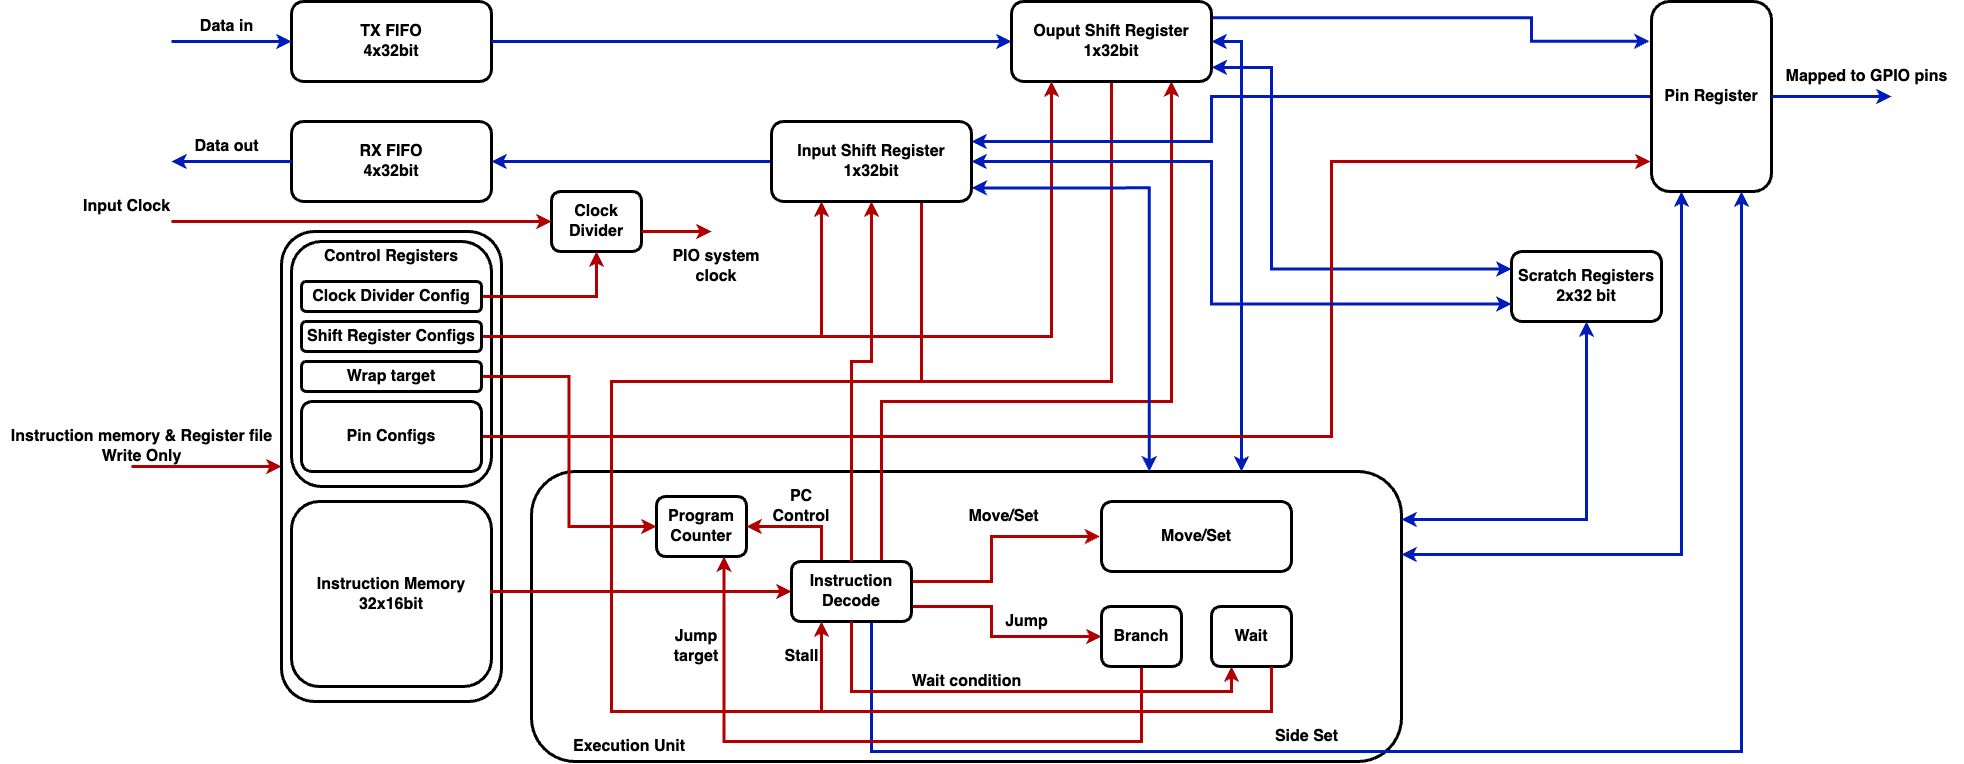
\includegraphics[width=1\textwidth]{../img/bd.png}
    \caption{Block diagram of the RVPIO device. A larger figure is given in Appendix \ref{ch:bd}.}
    \label{fig:bd}
\end{figure}

The primary datapath is that between the FIFOs and output pins via the shift registers: data is shifted from the pins into the ISR, and then pushed to the RX FIFO (and the same in reverse via the OSR). Execution of \txt{PUSH}, \txt{PULL}, \txt{IN}, and \txt{OUT} instructions is handled by logic within the shift registers themselves, controlled by signalling from the execution unit. The shift registers may signal a stall to the instruction decoder if attempting to push to a full/pull from an empty FIFO.

The other four instructions are executed in sub-units of the execution unit. \txt{MOVE} and \txt{SET} instructions can read/write to any of the 5 registers, the branch unit reads registers to compute branch conditions, and the wait unit reads the pin register to conditionally signal a stall back to the instruction decoder.

Much of the complexity in control signalling lies in the execution unit, as the instruction decoder and program counter have to be able to handle instruction stalling and re-execution, and inserting delays into the flow of execution. The instruction decoder also directly signals side-set values to the pin register.

The control registers and instruction memory form a single 16-bit address space which is accessible via a write-only memory port from the host system. All the control registers included are shown on the diagram. Enough memory is included for 32 instructions, same as the RP2040 PIO \cite{rp2040}. The control registers are all readable by the components which they configure.

From this starting point is easy to move to HDL implementation: each block defines a Chisel module, and the inputs and outputs for each module are already well defined.

\section{SoC template}

For designing the SoC, our starting point is a GitHub repository by Xilinx  engineer Eugene Tarassov\footnote{\url{https://github.com/eugene-tarassov/vivado-risc-v}}, providing scripts and source code to generate a RISC-V SoC based on Rocket chip in Vivado, Xilinx's FPGA design tool. A number of Xilinx boards are supported, including our Digilent Nexys A7 board. The block design from the Vivado project is shown in  \ref{fig:vivado-bd}.

As well as a Rocket Chip SoC with configurable functionality (primarily the number and type of cores), RTL modules are included for an Ethernet controller, SD card controller, and UART serial port, allowing to run a fully functional system with internet connectivity on the FPGA. The peripherals are external to the Rocket chip system and connected over an AXI network. AXI (Advanced eXtensible Interface) is part of ARM's Advanced Microcontroller Bus Architecture (AMBA), and provides a protocol for interconnect in digital systems designs. It is ubiquitous within Xilinx IP, and is also used within our system \cite{axi}.

This gives two options for integrating PIO: as part of the Rocket system, or as part of the AXI network. We do the latter, as AXI is much better documented than Rocket chip's interconnect mechanisms, and better supported within Xilinx's tools and ecosystem. The PIO module can be designed entirely separately, and then easily imported into the design as an extra RTL module using Vivado's block design tools, and mapped into the processor's address space using the address editor.

\begin{figure}[H]
    \centering
    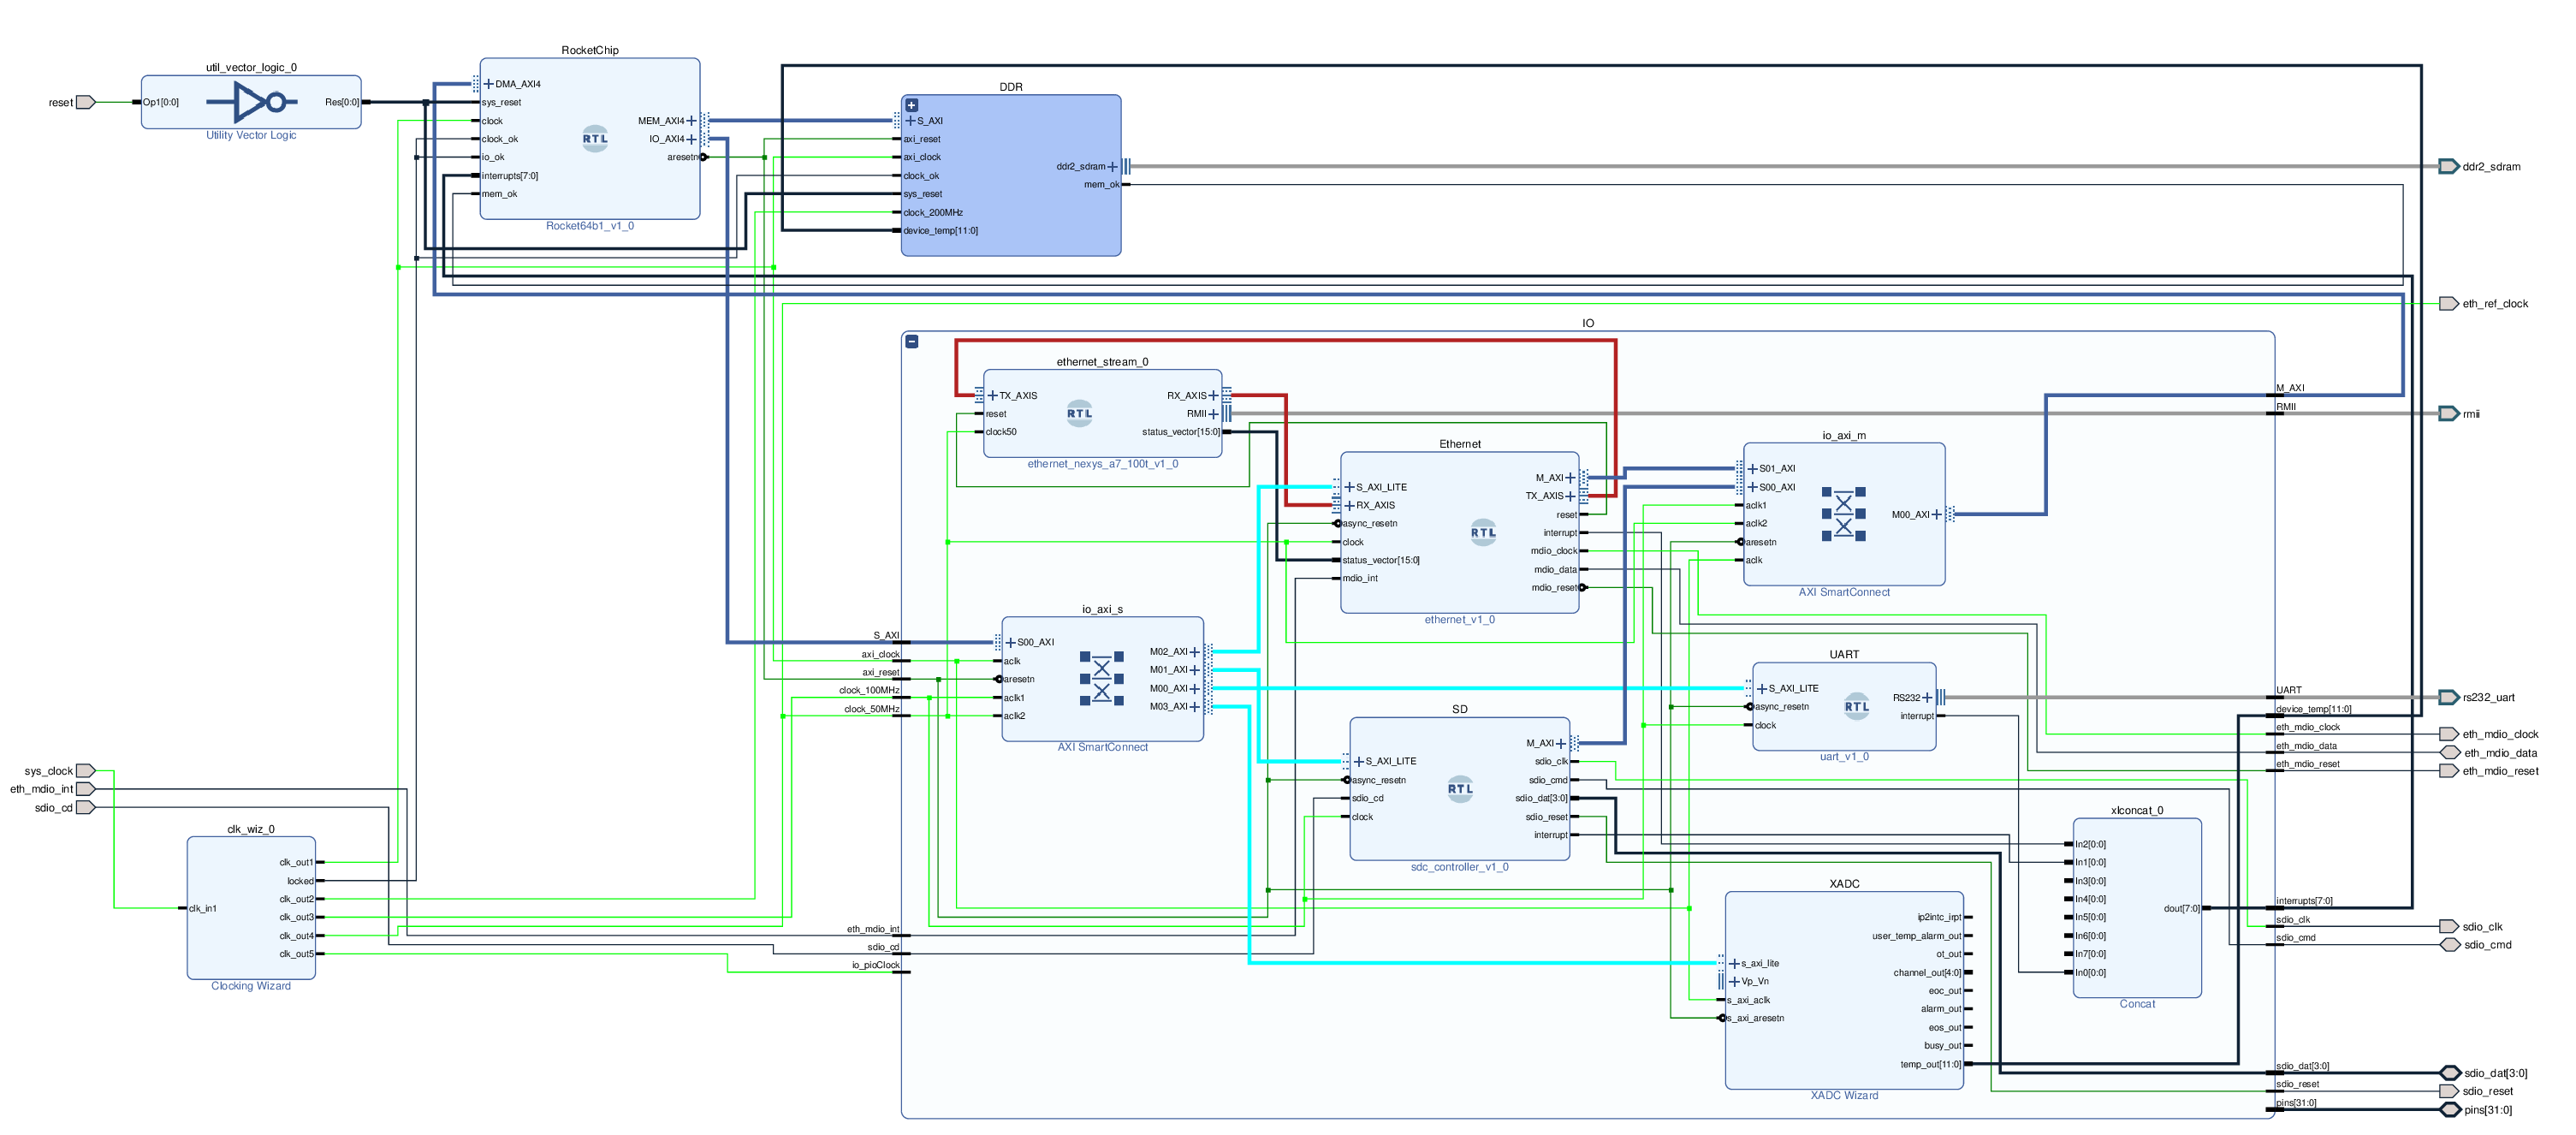
\includegraphics[width=1\textwidth]{../img/block-design.png}
    \caption{The Vivado block diagram which we integrate PIO into}
    \label{fig:vivado-bd}
\end{figure}

Scripts are provided for compiling the Linux kernel and a Debian-based system, which can be interacted with via a serial console. Alternatively, bare metal software can be compiled to run directly on the cores, for which a linker script and startup assembly code is provided. Software is loaded from an ELF executable on an SD card by a bootloader stored in RAM on the FPGA. Implementing Linux kernel drivers for PIO is out of scope for this project, so we target bare metal software for writing any test code.



